% LaTeX formatting example for NERCCS
% Revised on 8/23/2018 by Hiroki Sayama

\documentclass[12pt]{article}
\usepackage[letterpaper,margin=1in]{geometry}
\usepackage{times}
\usepackage{graphicx}
\usepackage{sectsty}
\allsectionsfont{\normalsize}
\usepackage{authblk}
\renewcommand\Authfont{\normalsize}

\begin{document}

\title{\normalsize\bf%
Understanding Reservoirs: Ideal Networks for Replicating Chaos}
\vspace{-0.5in}
\author{\vspace{-0.25in} J Jamieson, D. Passey, D. Smith,  B. Webb, and J. Wilkes\\
}

\date{\vspace{-5ex}} % to kill the unnecessary blank space for \date{}

\maketitle

\thispagestyle{empty}
\pagestyle{empty}


\normalsize \vspace{-.25in}

\begin{figure}[h]
\centering
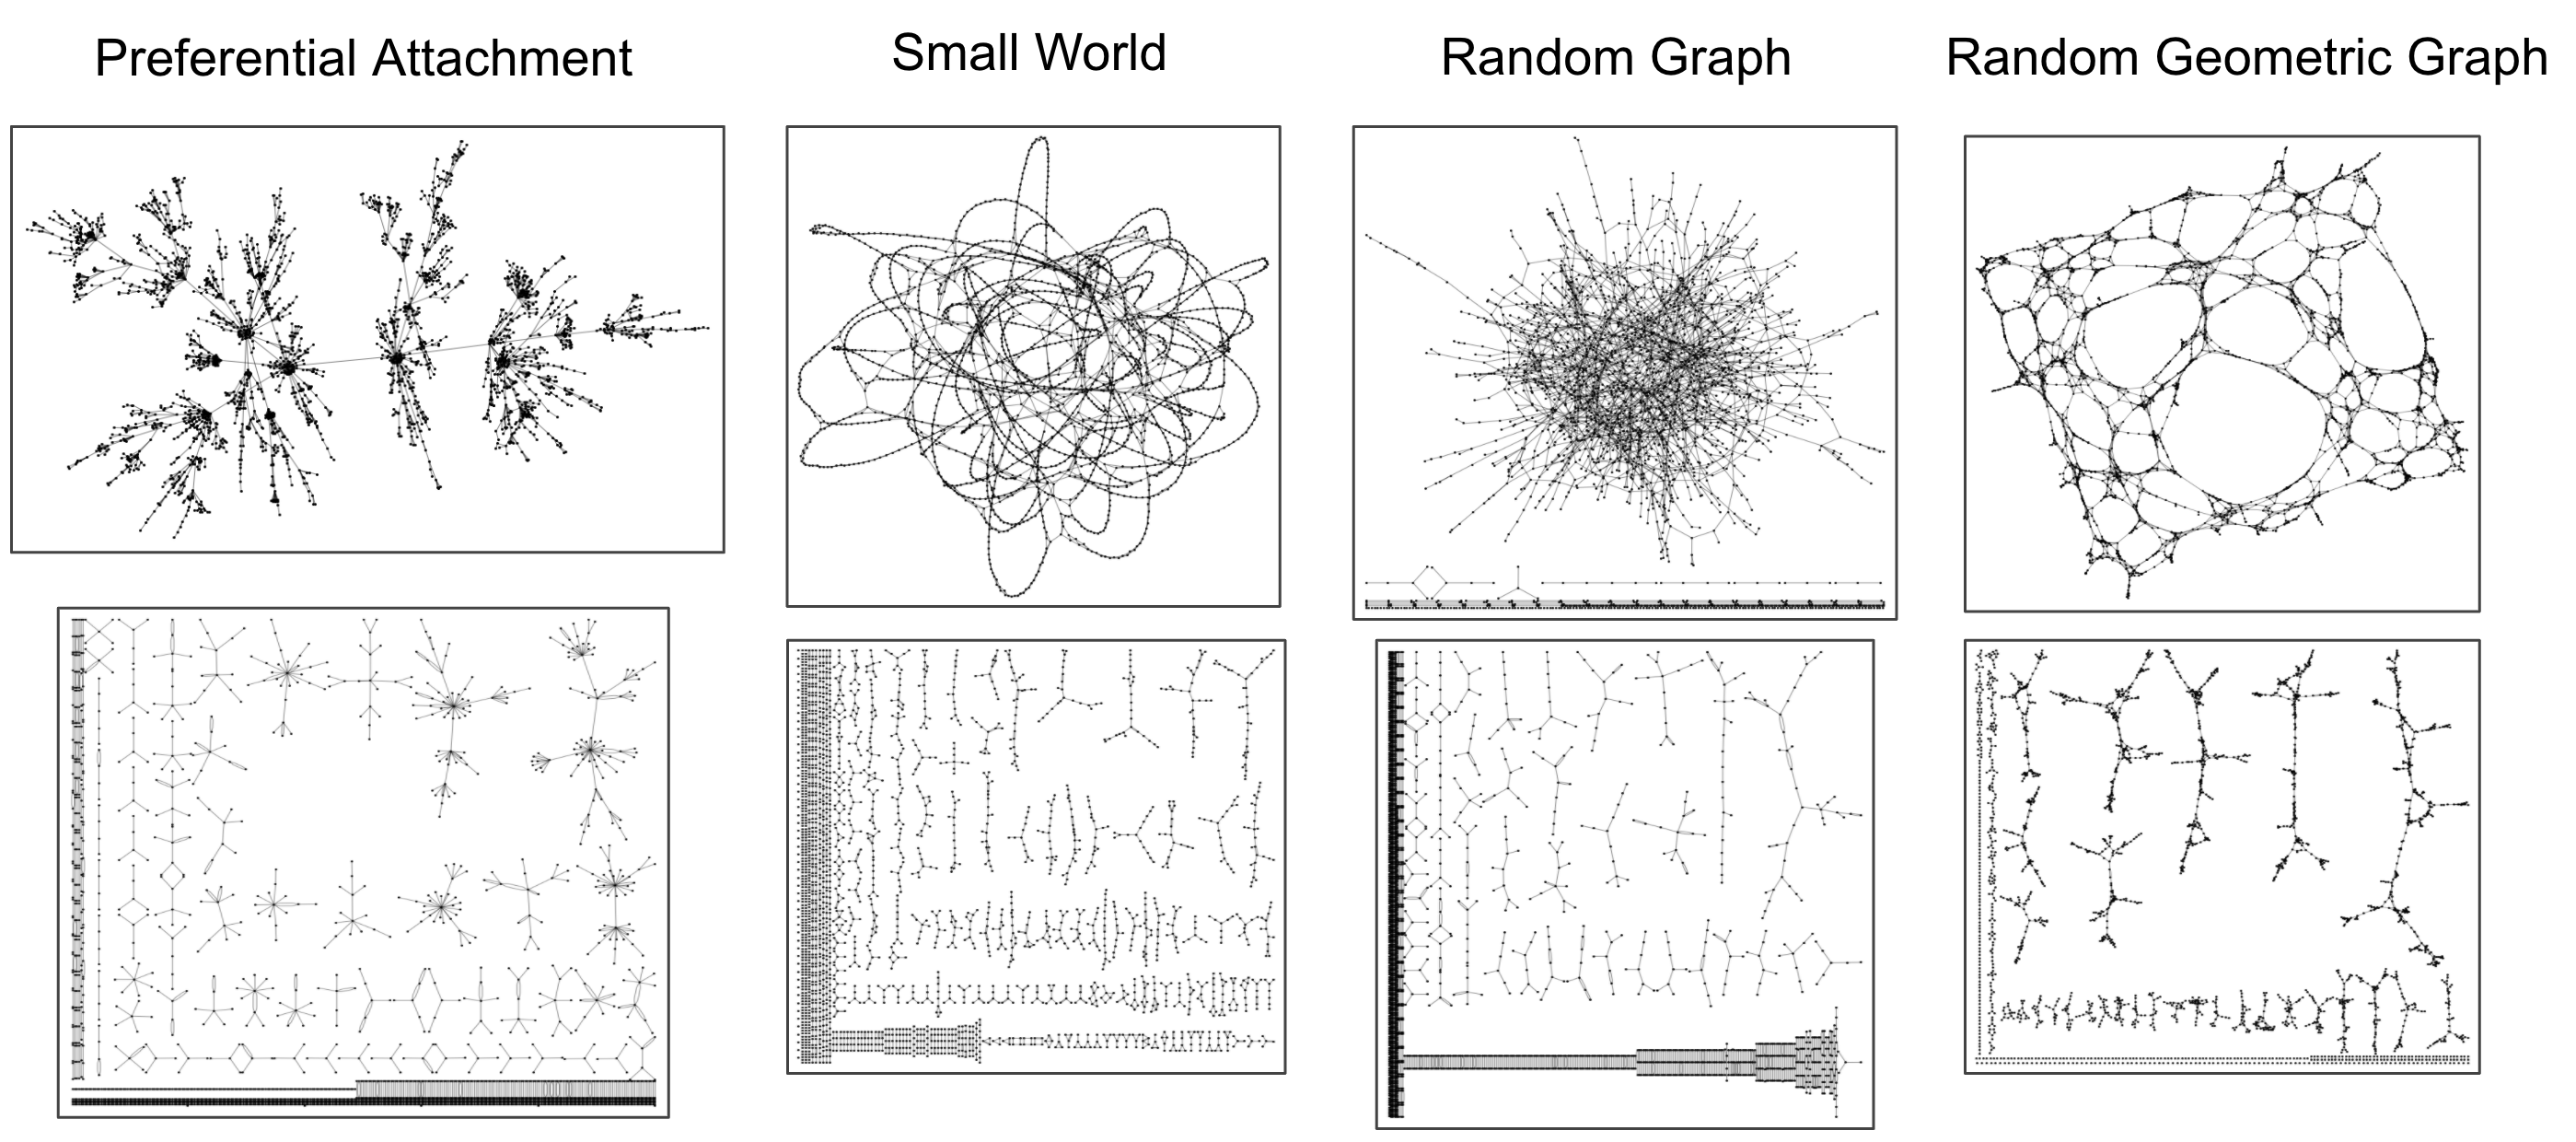
\includegraphics[width=.6\columnwidth]{networkthinning.png}
\caption{Complex network models before and after removing 80\% of the edges.}
\label{fig:nets}
\end{figure}
Reservoir computers are a machine learning model that, unlike most standard machine learning models, make use of an internal complex network \cite{review}. The effect of network topology on the dynamics of reservoir computers is not well understood. To investigate this, we trained over one-hundred million reservoir computers to replicate the chaotic dynamics of the Lorenz attractor. In our experiments, we varied hyperparameters and internal network structure to determine the combinations that produce the best predictions.

Specifically, we studied how reservoir computer prediction varied with respect to common network topologies across a substantial range of hyperparameters. We also studied the performance of "thinned" versions of the standard topologies, by removing a percent of edges at random.

We found that sparse, e.g. thinned, networks are typically better suited to learn the dynamics of the Lorenz attractor. Our experiments also revealed an interaction between the reservoir computer spectral radius parameter (a rescaling of the reservoir adjacency matrix to produce a desired spectral radius) and the sparsity of the internal network suggesting that spectral radius and sparsity combine in unexpected ways to impact reservoir computer predictive ability.

To help interpret our experimental findings, we analyzed the untrained reservoir dynamical system, studying how reservoir computer fixed points and their stability vary in response to a training signal. This analysis demonstrated that high spectral radius and high connectivity reduce the sensitivity of reservoir computers to input data, making them poorly suited for learning. This analysis offers insight into better design principles for reservoir computers and better understanding of the role of network topology in machine learning.



\begin{thebibliography}{9}
\bibitem{review} 
Tanaka, Gouhei, et. al. "Recent advances in physical reservoir computing: A review",
\textit{Neural Networks}, vol. 115. (2019).

\end{thebibliography}


\end{document}